\label{chapter:preditor}

This chapter presents \Predator{}, which improves the effectiveness of false sharing detection. \SheriffDetect{} reports false sharing accurately and precisely with only $20\%$ performance overhead. However, it can only detect the write-write type of false sharing for those programs using \pthreads{}. \SheriffDetect{} can also break programs that communicate across different threads using stack variables or self-defined synchronizations. These shortcomings greatly limit \SheriffDetect{}'s usage on real-world applications.  

In contrast to \SheriffDetect{}, \Predator{} detects all types of false sharing and has no limitations on applications. \Predator{} has been utilized to find actual false sharing problems of real applications, including \texttt{MySQL} and the \texttt{Boost} library.

In addition, \SheriffDetect{} and other systems share one key limitation: they can only report \emph{observed} cases of false sharing. As Nanavati et al.\ point out, false sharing is sensitive to where objects are placed in cache lines and so can be affected by a wide range of factors~\cite{OSdetection}. For example, using the gcc compiler \emph{accidentally} eliminates false sharing of the linear\_regression benchmark at certain optimization levels, while LLVM does not do so at any optimization level.  A slightly different memory allocation sequence (or different memory allocator) can reveal or hide false sharing, depending on where objects end up in memory; using a different hardware platform with different addressing or cache line sizes can have the same effect. All of this means that existing tools cannot root out potentially devastating cases of false sharing that could arise with different inputs, in different execution environments, and on different hardware platforms.

\Predator{} is the first system that can \emph{predict} potential false sharing that does not manifest in an execution, but may appear and greatly degrade the performance of programs in a slightly different environment. Predictive false sharing generalizes from a single execution to identify potential false sharing instances that fall into two adjacent cache lines, which could be exposed by slight changes in object placement and alignment. It also can predict false sharing in hardware platforms with larger cache line sizes by tracking accesses within \emph{virtual cache lines} that span multiple physical lines. Predictive false sharing detection thus help avoids the predicament of previous detection tools: those problems can easily leak to deployment environment because of the changed execution environment.

Here, we first describe \Predator{}'s false sharing detection mechanism in Section~\ref{sec:detection}, which consists of both compiler and runtime system components. Section~\ref{sec:prediction} then explains how \Predator{} predicts potential false sharing based on a single execution.

\section{False Sharing Detection}
\label{sec:detection}

\subsection{Overview}
\label{sec:overview}
\Predator{} follows the same idea of detecting false sharing, described in Section~\ref{sec:detectionidea}. We compute cache invalidations based only on memory accesses history of each cache line, and only report those instances that may affect performance. 

\Predator{} is based on the similar {\it basic observation}: if a thread writes a cache line after other threads have accessed the same cache line, this write operation causes at least a cache invalidation. Drawing from this observation, \Predator{} tracks cache invalidations of all cache lines and ranks the severity of performance degradation  according to the number of cache invalidations. 
% by keeping track of accesses from different threads. 
 
To track memory accesses, \Predator{} relies on the compiler instrumentation. The design tradeoff of choosing compiler instrumentation, instead of other mechanisms, has been discussed in Section~\ref{sec:instrumentationtradeoff}. A compiler can easily identify read or write accesses. However, a compiler does not know how and when those instructions are being executed, since that depends on a specific execution, input, and runtime environment.

Therefore, \Predator{} combines a runtime system with compiler instrumentation to track cache invalidations: the compiler instruments memory accesses so the runtime system is notified when an access is executed (see Section~\ref{sec:compiler}), and the runtime system is responsible for collecting and analyzing actual memory accesses to detect and report false sharing (see Section~\ref{sec:runtime}).

\subsection{Compiler Instrumentation}
\label{sec:compiler}

\Predator{} relies on LLVM to perform instrumentation at the intermediate representation level~\cite{llvm}.
It traverses all functions one by one and searches for memory accesses to those global and heap variables.  For each memory access, \Predator{} instruments a function call to invoke the runtime system, passing with the address, access type and unit of this memory access (how many bytes). \Predator{} currently omits accesses to stack variables by default because stack variables are normally used for thread local storage and therefore do not normally introduce false sharing. However, instrumentation on stack variables
can always be turned on when necessary.

The instrumentation pass is placed at the very end of the LLVM optimization passes so that only those memory accesses surviving all previous LLVM optimization passes are instrumented.  This technique is similar to the one used by AddressSanitizer~\cite{AddressSanitizer}.

\subsection{Runtime System}
\label{sec:runtime}

\Predator{}'s runtime system collects every memory access by handling those functions calls inserted during the compiler instrumentation phase. It analyzes possible cache invalidations based on the basic observation discussed in Section~\ref{sec:overview}. Finally, it precisely reports any performance-degrading false sharing problems it finds.  For global variables involved in false sharing, \Predator{} reports their name, address and size; for heap
objects, \Predator{} reports the callsite stack for their allocations, address and size. In addition, \Predator{} provides word granularity access information for those cache lines involved in false sharing: how many reads or writes are issued by which thread.  This information can further help users diagnose and fix false sharing instances.

\subsubsection{Tracking Cache Invalidations}
\Predator{} only reports those global variables or heap objects on cache lines with a large number of cache invalidations, thus possibly affecting performance of applications. To track cache invalidations, \Predator{} maintains a two-entries-cache-history table for each cache line.  In this table, each entry has two fields: thread ID and access type (read or write). Thread ID is used to identify the origin of each access. As stated earlier, only accesses from different threads (with a different thread ID) can cause a cache invalidation.

For every new access to a cache line $L$, \Predator{} checks $L$'s history table $T$ to decide whether the current access leads to a cache invalidation.  As described in Section~\ref{}, only write accesses can cause cache invalidations and read accesses only create a copy of data in the cache of the current core that the current thread is running on. Also, it is noticed that table $T$ only has two status: full and not full.  There is no ``empty'' status since every cache invalidation should replace its table with the current write access, setting the first entry to the current access (with its thread ID and write access type).

\begin{itemize}
\item
  For a read access $R$, 
  \begin{itemize}
    \item
      If $T$ is full, there is no need to record this read access.
    \item
      If $T$ is not full and another existing entry has a different thread
      ID, then \Predator{} records this $R$ (and its thread) by adding a new entry to the table. 
  \end{itemize}
\item
  For a write access $W$, 
  \begin{itemize}
    \item
      If $T$ is full, then $W$ can cause a cache invalidation since at least one of two existing accesses are issued by a different thread (one thread can only occupy one entry).
      After recording this invalidation, \Predator{} updates the existing entry with $W$(and its thread).
    \item
      If $T$ is not full,
      \Predator{} checks whether $W$ and the existing entry has the same thread ID. If so, $W$ cannot cause a cache invalidation and there is no need to do anything. Otherwise, \Predator{} identifies a possible cache invalidation on this line: it increments the number of cache invalidations and updates the existing entry with the current $W$ access.
  \end{itemize}
\end{itemize}

\subsubsection{Reporting False Sharing}
\label{sec:predatorcallsite}

\Predator{} reports false sharing precisely and accurately. Accurately means \Predator{} only reports those false sharing instances with a large number of cache invalidations, which may possibly cause performance problems. \Predator{} also differentiate actual false sharing from true sharing, since true sharing can also induce a large number of cache invalidations.

\Predator{} employs the following mechanisms to achieve this target, as well as reducing the performance overhead.  

\begin{itemize}
\item

In order to accurately differentiate those false sharing problems with true sharing problems, \Predator{} tracks word-level accesses for those cache lines involved in a big number of cache invalidations, which has been discussed in Section~\ref{sec:accuratedetect}.


\item
\predator{} relies on \texttt{backtrace()} function in the \texttt{glibc} library to obtain the whole callsite stack, which is slower but much more robust to be used than the ways used in \SheriffDetect{}. Thus, it can report the callsite stack for those heap objects. 


\item
For every access, \Predator{} needs to lookup the corresponding cache line's metadata. Because this operation is so frequent, at every access, lookups need to be very efficient. Like AddressSanitizer~\cite{AddressSanitizer} and other systems~\cite{Valgrind, qinzhao}, \Predator{} uses a shadow memory mechanism to store metadata for every piece of application data.  Thus, \Predator{} can compute and locate corresponding metadata directly via address arithmetic.

\item
In order to support shadow memory, \Predator{} uses a pre-defined starting address and fixed size for its heap.  It also contains a custom memory allocator, which is described in Section~\ref{sec:customheap}.  However, using this custom memory allocator also implies that false sharing caused by a memory allocator cannot be detected by \Predator{}: two threads allocate heap objects from the same cache line concurrently. But this should not be a serious problem since  all modern memory allocators, like Hoard, already avoid this kind of false sharing and we should always use this kind of memory allocator.

\end{itemize} 
 
\subsection{Optimizations}
\label{optimization}
Tracking every memory access can be extremely expensive, thus \Predator{} utilizes the following mechanisms to further reduce performance and memory overhead.

\subsubsection{Threshold-Based Tracking Mechanism}
\label{sec:thresholdtracking}
\Predator{} aims to detect false sharing that significantly degrades performance. Since cache invalidations are the root cause of performance degradation and only writes 
can possibly cause cache invalidations, 
cache lines with a small number of writes are never be a target with a significant performance impact.
For this reason, \Predator{} only tracks cache invalidations
once the number of writes to a cache line crosses a
pre-defined threshold, which we refer to as the {\it Tracking-Threshold}. 
Before this threshold is reached, \Predator{} only tracks the number of writes on a cache line while skipping tracking reads. This mechanism reduces performance and memory overhead
at the same time.

In the current implementation, \Predator{} maintains two arrays in shadow memory: 
{\it CacheWrites} tracks the number of memory writes on every cache line, and
{\it CacheTracking} tracks detailed information 
for each cache line once the number of writes on a cache line exceeds the {\it Tracking-Threshold}. 
If the threshold is not reached, there is no need to check the corresponding {\it CacheTracking}. 
Figure~\ref{fig:algorithm} illustrates the detailed mechanism.

\begin{figure}[!t]
\begin{lstlisting}[style=tt]
void HandleAccess(unsigned long addr, bool isWrite) {
 unsigned long cacheIndex=addr>>CACHELINE_SIZE_SHIFTS;
 cachetrack *track=NULL;

 if(CacheWrites[cacheIndex]<TRACKING_THRESHOLD) {
  if(isWrite) {
   if(ATOMIC_INCR(&CacheWrites[cacheIndex]) 
      ==TRACKING_THRESHOLD-1) {
     track=allocCacheTrack();
     ATOMIC_CAS(&CacheTracking[cacheIndex],0,track));
   }
  } 
 }
 else {
  track=CacheTracking[index]);
  if(track){
    // Track cache invalidations and detailed accesses
    track->handleAccess(addr, isWrite);
  }
 }
}
\end{lstlisting}
\caption{Pseudo-code of handling an access in \Predator{}.\label{fig:algorithm}}
\end{figure}

To avoid expensive lock operations, \Predator{} uses atomic instruction to increment the {\it CacheWrites} counter for each cache line. 
When the number of writes of a cache line reaches the predefined threshold,
it allocates space to track detailed cache invalidations and word-level information. \Predator{} also 
uses an atomic compare-and-swap to set the cache tracking address for this cache line in the shadow mapping.
After {\it CacheWrites} on a cache line reaches the {\it Tracking-Threshold}, all read and write accesses on this cache line are tracked.


\subsubsection{Selective Compiler Instrumentation}
\label{sec:selectinstrumentation}

\Predator{} relies on compiler instrumentation to provide memory access information to the runtime system 
and detects false sharing based on the sequences of memory accesses on every cache line. 
The performance overhead of a specific program is always proportional to the degree of instrumentation: more instrumentation generally indicates more performance overhead. 
Thus, \Predator{} provides a flexible framework to instrument programs depending on the performance requirements of the user.

Currently, \Predator{} only instruments once for each type of memory access on each address 
to the same basic block. 
This selective instrumentation does not normally affect the effectiveness of detection. 
Because \Predator{} aims to detect false sharing cases with a large number of cache invalidations,
less tracking of accesses inside a basic block can induce fewer cache invalidations, but it should not affect the overall behavior of cache invalidations. 

% detection will not cause performance problem. 
To improve performance further,
\Predator{} can be easily extended to support more flexible instrumentation as follows:
\begin{itemize}
\item
\Predator{} could selectively instrument both reads and writes or only writes.
Instrumenting only writes reduces overhead while detecting write-write false sharing, 
as \Sheriff{} does. 
\item
\Predator{} can be set to instrument or skip specific code or data. 
For example, the user could provide a black-list so that given modules,
functions or variables are not instrumented. 
Conversely, the user could provide a white-list so that only specified functions or variables are instrumented. 
\end{itemize}

\subsubsection{Sampling Mechanism}
\label{sec:sample}
As described in Section~\ref{sec:thresholdtracking}, when the number of writes on a cache line is larger than {\it Tracking-Threshold}, every
access must be tracked in detail: we have to track word-level 
information, update the number of accesses and possible cache invalidations, and update the cache access history table
of this cache line.  When a cache line is involved in false or true sharing, updating those counters can exacerbate the performance impact of sharing: not only is there an cache invalidation on this application's cache line, but there is also at least another cache invalidation caused by updating the metadata of this corresponding cache line.

To further reduce the performance overhead, \Predator{} only samples the first specified number of accesses during each sampling interval. 
Currently, \Predator{} maintains an access counter for each cache line
and only tracks the first $10,000$ accesses out of every 1 million accesses on a cache line, with 1\% sampling rate. Section~\ref{sec:predatorsensitivity} further evaluates the effect of different sampling rates on performance and effectiveness.  



\section{False Sharing Prediction}
% Why prediction is important?
\label{sec:prediction}
This section further motivates predictive false sharing and explains how to support it in the runtime system.  

\subsection{Overview}
%\begin{figure*}[!htb]
\label{sec:predictoverview}

\begin{figure}[!t]
\begin{center}
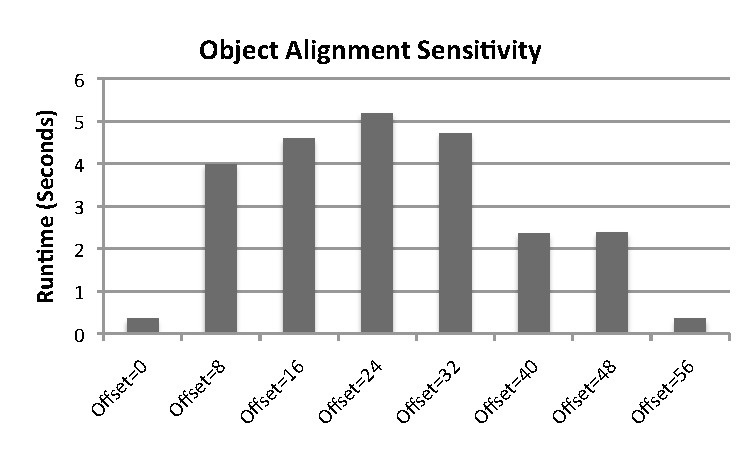
\includegraphics[width=6in]{predator/figure/perfsensitive}
\end{center}
\caption{
Performance of the linear\_regression benchmark (from Phoenix)  is highly sensitive to the memory layout between the (potentially) falsely-shared object and corresponding cache lines. 
\label{fig:perfsensitive}}
\end{figure}

The appearance of false sharing depends on 
the memory layout between objects and corresponding cache lines. The performance of a real example, linear\_regression, is shown in Figure~\ref{fig:perfsensitive}: 
When the offset of the starting address between the potentially falsely-shared object and corresponding cache lines is $0$ or $56$ bytes, there is no false sharing; 
When the offset is $24$ bytes, we see the most severe performance effect caused by false sharing. 
The performance difference caused by false sharing can affect the performance as large as $15\times$ on an 8-core machine. 

Existing detection tools can only report observed false sharing. That means, they may miss such a very severe false sharing problem that could occur in the wild if the offset of the starting address was $0$ bytes or $56$ bytes in their test environment. \Predator{} overcomes this shortcoming by accurately predicting potential false sharing, without the need of occurrences. 

\begin{figure*}
\begin{center} 
\subfigure[No false sharing]{%
   \label{fig:nofs}
   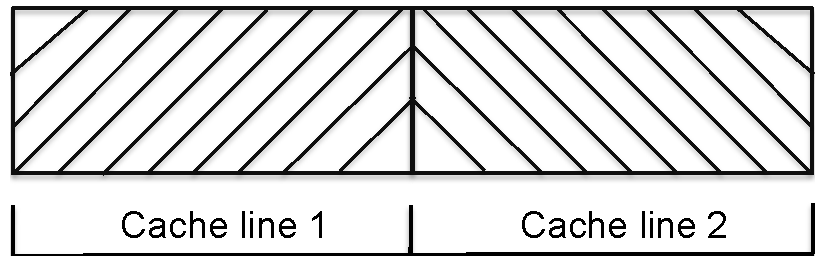
\includegraphics[width=0.24\textwidth]{predator/figure/Potential1}
}%
\hspace{10pt}
\subfigure[False sharing with larger cache size]{%
   \label{fig:fslarger}
   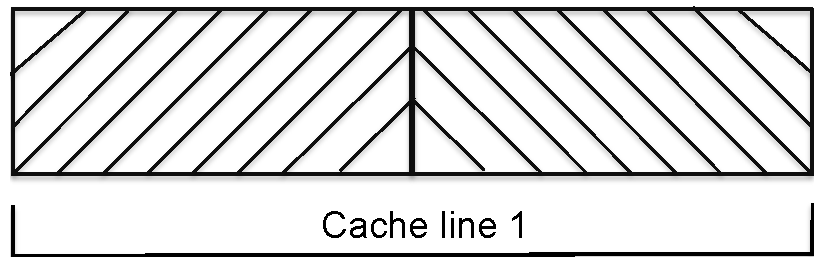
\includegraphics[width=0.24\textwidth]{predator/figure/Potential2}
}%
\hspace{10pt}
\subfigure[False sharing with different memory layout]{%
   \label{fig:fsnoalignment}
   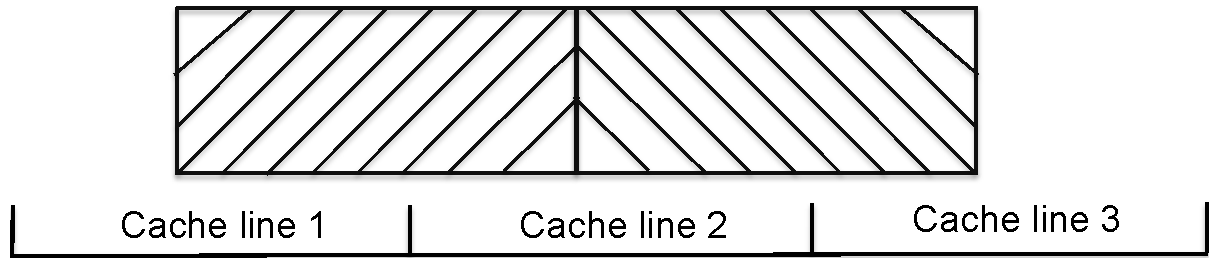
\includegraphics[width=0.36\textwidth]{predator/figure/Potential3}
}%
\end{center}
%\includegraphics{fig/potential.pdf}
\caption{False sharing under different environments.}
\label{fig:potentialfalsesharing}
\end{figure*}

\Predator{} predicts {\it potential false sharing}, which does not manifest in the current execution but may appear and greatly affect performance of programs in a slightly different environment.

Figure~\ref{fig:potentialfalsesharing} shows a simplified example why occurrences of false sharing can change in different situations. 
In this figure, two rectangles with different patterns
represents two portions of the same object, updated by different threads. In Figure~\ref{fig:nofs}, there is no false sharing when thread T1 only updates 
``cache line 1'' and T2 only updates ``cache line 2''.
However, false sharing appears in one of the following cases, even with the same
access pattern. 

\begin{itemize}
\item
Doubling cache line size (Figure~\ref{fig:fslarger}). When the size of a cache line doubles, both T1 and T2 access the same cache line concurrently, thus causing false sharing.

\item
Different starting address of an object(Figure~\ref{fig:fsnoalignment}).  
When the starting address of this object is not aligned with the starting address of the first cache line, then T1 and T2 can update the second cache line simultaneously, causing a false sharing problem. 
%When some dynamic property changes the starting address of this object so that it 
%is not aligned with the starting address of the first cache line, 
\end{itemize} 

\Predator{} predicts whether programs can have potential false sharing in one of these two situations, where they can be caused by different dynamic properties. These dynamic properties include choosing a different compiler, enabling different compiler optimizations, using a different memory allocator, adding or removing code involving in memory allocations, switching to a different target platform with a different address mode (32-bit or 64-bit), and changing the size of cache line (64 Bytes or 128 Bytes). 
All dynamic properties, except changing the size of cache line, can lead to a different memory layout, thus can possibly affect occurrences of a false sharing problem. Thus, predicting false sharing in changing the memory layout or changing the size of cache line actually explores many possibilities caused by all of these dynamic properties.

\subsection{Basic Prediction Workflow}
\label{sec:predictionmechanism} 

%Similar to the detection part, 
\Predator{} focuses on potential false sharing that can 
cause performance problems.
It is based on two key observations. First, only accesses to 
adjacent cache lines can lead to potential false sharing, 
i.e., introducing cache invalidations when the cache line size
or an object's starting address changes.
Second, only those cache lines with a large number of cache invalidations can degrade performance.

Based on these two observations, \Predator{} develops 
the following workflow to predict potential false sharing.
Those detection optimizations listed in Section~\ref{optimization} can also be applied
to here. We do not repeat these optimizations in this section.

\begin{enumerate}
\item
Track the number of writes on different cache lines. 

\item
When the number of writes to a cache line $L$ reaches {\it Tracking-Threshold},
\predator{} tracks the detailed read and write accesses for every word on both cache line $L$ 
and its adjacent cache lines. 

\item
When the number of writes to a cache line $L$ reaches a second threshold (called as
{\it Predicting-Threshold}), 
\predator{} identifies whether there exists false sharing in $L$ and its adjacent cache lines by analyzing word accesses information collected in Step 2, which are described in 
Section~\ref{sec:evaluatingfs} in detail.

\item
If a potential false sharing is found, \predator{} starts to track cache line invalidations in order to confirm its seriousness, which are discussed in Section~\ref{sec:tracking}.
Otherwise, go back to Step 2 to track more detailed accesses.
 
\end{enumerate}

\subsection{Searching for Potential False Sharing}
\label{sec:evaluatingfs}
To describe potential false sharing in two different cases, we first introduce a concept -- ``virtual cache line''.  A virtual cache line is a contiguous memory range that spans one or more physical cache lines.  

In the case of double cache line size, a virtual line is composed of two originally contiguous cache lines, where it starts with a even number cache line.  Thus, only cache lines $2*i$ and $2*i+1$ can form a virtual cache line.  

To evaluate a potential false sharing problem that can be caused by changing memory layout, a virtual line should have the same size as an actual cache line, but with a different starting address: unlike actual cache lines, the
starting address of a virtual cache line does not need to be multiple of the cache line size. For instance, a 64-byte-long virtual line can consist of the range $[0,64)$ bytes or $[8,72)$ bytes.

To search for a potential false sharing problem, 
\Predator{} searches for a pair of hot accesses, one on $L$ and one on its previous or next cache line, based on detailed word information collected in Step 2. Two accesses happening in the same actual cache line should be detected by the normal detection mechanism, thus they can lead to actual false sharing problems but not a potential false sharing problem. 

A hot access refers to an access that has the number of read or write accesses larger than the average number of accesses. In fact, for every hot access $X$ in a specific cache line $L$, \Predator{} searches another
hot access $Y$ in $L$'s previous cache line or next cache line, satisfying the following conditions: 

\begin{itemize}
\item
$X$ and $Y$ reside on the same virtual line. 

\item
One of $X$ and $Y$ is a write access.

\item 
$X$ and $Y$ are issued by different threads.

\end{itemize}

% why it finds a pair of $X$ and $Y$ == a potential false sharing 
Whenever it finds such a pair, $X$ and $Y$, 
\Predator{} identifies a potential false sharing problem: they can degrade performance when the number of cache invalidations possibly caused by $X$ and $Y$ (on a possible virtual line), is larger than a pre-defined threshold. This approach is based on a similar observation as in detection: \emph{if a thread writes a virtual line after other threads have accessed the same virtual line, this write operation causes at least one cache invalidation}. 

However, before tracking detailed memory accesses on a specific virtual line, it is impossible to know exactly how many cache invalidations actually happen on this virtual line. Thus, \Predator{} conservatively assumes that accesses from different threads occurs in a interleaved way, with the maximum number of cache invalidations. Then \Predator{} starts to track possible cache invalidations on a virtual covering both $X$ and $Y$, described in Section~\ref{sec:tracking}.  

%According to above observation and assumption, 
%a pair of hot accesses, $X$ and $Y$, if accesses are issued in an interleaving 
%way, can generate the number of cache invalidations equaling to 
%the smaller number of accesses of $X$ and $Y$.
%Thus a false sharing problem is to be identified by \Predator{}.
  

\subsection{Verifying Potential False Sharing}
\label{sec:tracking}

\Predator{} verifies potential false sharing by tracking possible cache invalidations on a specific virtual line covering such a hot access pair, $X$ and $Y$.
%covering a pair of hot accesses found
%in Step 3.

For potential false sharing caused by double cache line size, as described in Section~\ref{sec:evaluatingfs}, a virtual line is always composed of cache line with index $2*i$ and $2*i+1$. 
\Predator{} tracks cache invalidations on a virtual line that covering $X$ and $Y$. This virtual line is unique for a given $X$ and $Y$ pair. 

However, for the case of changing memory layout, two hot accesses with distance less than the cache line size 
can actually form multiple virtual lines. 
There is thus an additional step to determine which virtual line to be tracked. 
Although a virtual line to be chosen here is never a real cache line of actual hardware because of unaligned addresses,
we utilize this virtual line to simulate the effect of changing memory layout correspondingly.


\begin{figure}
\begin{center} 
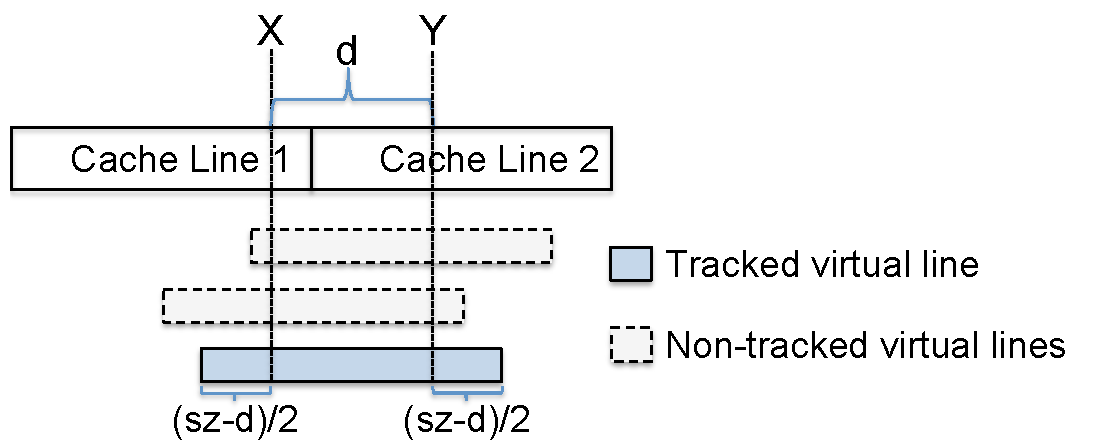
\includegraphics[width=6in]{predator/figure/trackpotential}
\end{center}
\caption{Determining a virtual line with size $sz$ according to hot accesses.}
\label{fig:trackpotential}
\end{figure}

Figure~\ref{fig:trackpotential} shows that multiple virtual lines can cover $X$ and $Y$. However, \Predator{} only chooses one of these virtual lines. \Predator{} chooses the virtual line that leaves the same space before $X$ and after $Y$. That is, the virtual line starting at location $X-((sz-d)/2)$ and ending at $Y+((sz-d)/2)$ is tracked by \Predator{}. This choice allows tracking of more possible cache invalidations caused by adjacent accesses of $X$ and $Y$. Since adjusting the starting address of a virtual line has the same effect of adjusting the starting address of an object in detecting false sharing, all cache lines related to the same object must be adjusted at the same time. \Predator{} then tracks cache invalidations based on these adjusted virtual lines.

In the end, \Predator{} can report accurately whether the change of memory layout can affect the performance or not, based on the possible number of cache invalidations. 

Currently, \predator{} only determines a specific virtual line to be tracked. However, we plan to extend this in the future work by using a much more flexible mechanism: we can choose a different virtual line after a number of accesses if the current choose cannot reveal a big number of cache invalidations.



\section{Evaluation}



\label{sec:evaluation}

This section answers the following questions:
\begin{itemize}
\item
  How effective is \Predator{} at detecting and predicting false sharing?

\item
  What is \Predator{}'s overhead, in terms of execution time and memory ?

\item
  How sensitive is \Predator{} to different sampling rates?
 
\end{itemize}

\paragraph{Experimental Platform.} All evaluations are performed on a quiescent Intel Core 2 dual-processor system,  equipped with 16GB RAM in total. Each processor is a 4-core 64-bit Intel Xeon running at 2.33 GHz, with a 4MB shared L2 cache and 32KB private L1 cache. The underlying operating system is an unmodified CentOS 5.5, running with Linux kernel version 2.6.18-194.17.1.el5. The glibc version is 2.5. 

\paragraph{Evaluated Applications.}
This paper evaluates two popular benchmark suites,
Phoenix (with large input) ~\cite{phoenix-hpca} and PARSEC (with simlarge input) ~\cite{parsec}. Even with unmodified LLVM-3.2, Facesim cannot be compiled successfully (having complaints on an undefined template) and Canneal aborts unexpectedly. Thus, these two benchmarks are excluded.
We also evaluate \Predator{} on six real applications, including MySQL, Boost, Memcached, aget, pbzip2 and pfscan.



\subsection{Detection and Prediction Effectiveness}
\label{sec:predatoreffective}

\begin{figure*}[htb]
{\centering
\tiny
\subfigure{\lstinputlisting[numbers=none,frame=none,boxpos=t]{predator/figure/linearregression.report}}
\caption{An example reported by \Predator{}, indicating a potential false sharing problem in the linear\_regression benchmark.
\label{fig:lrreport}}
}
\end{figure*}

For every false sharing problem, \Predator{} reports source code information and detailed memory access information in order to help users fix those problems. Figure~\ref{fig:lrreport} shows an example for the linear\_regression benchmark. This report shows that the heap object starting with $0x40000038$ potentially causes a large number of cache invalidations. The call stack of this memory allocation is provided to help locate culprits. In addition, \Predator{} also reports word-level access information of this object, which helps to identify where and how false sharing occurs. From that, we can know that it is a latent false sharing problem predicted by \Predator{}, since different threads are accessing different cache lines. 

\subsubsection{Benchmarks}
\label{sec:benchmarks}

\begin{table}[!t]
{\centering
\resizebox{\columnwidth}{!}{
\begin{tabular}{l|r|r|r|r|r}\hline
{\bf \small Benchmark} & {\bf \small Source Code} & {\bf \small New} & {\bf \small Without Prediction} &{\bf \small With Prediction} & {\bf \small Improvement} \\
\hline
\small \textbf{histogram} & {\small histogram-pthread.c:213} & \cmark{} &\cmark{} & \cmark{} & 46.22\%\\
\small \textbf{linear\_regression} & {\small linear\_regression-pthread.c:133} & & & \cmark{} & 1206.93\% \\
\small \textbf{reverse\_index} & {\small reverseindex-pthread.c:511} & & \cmark{} & \cmark{} & 0.09\%\\
\small \textbf{word\_count} & {\small word\_count-pthread.c:136} & & \cmark{} & \cmark{} & 0.14\%\\
\hline
\small \textbf{streamcluster} & {\small streamcluster.cpp:985} &  & \cmark{} & \cmark{} &7.52\% \\
\small \textbf{streamcluster} & {\small streamcluster.cpp:1907} & \cmark{} & \cmark{} & \cmark{} & 4.77\%\\
\hline
\end{tabular} }
\caption{False sharing problems in the Phoenix and PARSEC benchmark suites. \label{table:detection}}
}
\end{table}

We evaluate \Predator{}'s effectiveness on two benchmark suites, Phoenix and PARSEC, and Table~\ref{table:detection} presents those benchmarks with false sharing problems. 
The first column lists those programs with false sharing problems.  The second column shows precisely where the problem is. Because all discovered false sharing occurs inside heap objects, we show the source code information of callsite here.  The third column, ``New'', marks whether this false sharing was newly discovered by \Predator{}.  A checkmark in the  following two columns indicates whether the false sharing was identified without prediction or with prediction enabled.  The final column, ``Improvement'', shows the performance improvement after fixing false sharing. Note that the performance improvement shown here is different with that in Table~\ref{table:perfafterfix} because \SheriffDetect{} evaluates on a 32bit platform and \Predator{} evaluates on a 64bit platform. This also shows that performance effect is every sensitive to hardware platform, which is one of dynamic properties that we discussed above. 
%The number is based on the average runtime of $10$ runs. 

As shown in the table, \Predator{} reveals two unknown false sharing problems. It is the first tool to uncover false sharing in histogram and at line $1907$ of streamcluster. 
In histogram, multiple threads simultaneously modify different locations of the same heap object, thread\_arg\_t. 
Padding this data structure fixes the false sharing problem and improves the performance by around 46\%. In streamcluster, multiple threads are simultaneously accessing and updating the same \texttt{bool} array, switch\_membership. Simply changing all elements of this array to a long type reduces the false sharing effect, improving performance by about 4.7\%.

%, although it is not a complete fix of false sharing. 
%None of these two false sharing problems has been reported by previous tools.
Other false sharing problems were discovered by previous work~\cite{sheriff}. The detailed reason of false sharing problems and how they are fixed are discussed in Section~\ref{sec:effecteval}.

It is worth noting that linear\_regression has a potential false sharing problem according to the execution environment of \Predator{}. According to the observation of Nanavati et al., this false sharing problem occurs when using clang and disappears when using gcc with the -O2 and -O3 optimization level~\cite{OSdetection}. But we observed a different result: when we are using the clang-3.2 compiler and our custom memory allocator, the false sharing problem does not occur at all because the offset happens to be 56 bytes (see Figure~\ref{fig:perfsensitive}). 
However, it does occur in the original execution environment, with the default memory allocator and using gcc compiler. That is why fixing it improves the performance by more than $12\times$.  This also exemplifies the necessity of \Predator{} predictive detection: existing tools may miss a false sharing problem if it does not occur at their test environments. 
 
\subsubsection{Real Applications}
To verify \Predator{}'s practicality, we further evaluate several widely-used real applications, whereas no previous work has done this. These real applications include a server application (MySQL~\cite{mysql}),
a standard C++ library (Boost~\cite{libfalsesharing}),
a distributed memory object caching system (Memcached), a network retriever (aget),
a parallel bzip2 file compressor (pbzip2), and a parallel file scanner (pfscan).

MySQL-5.5.32 and boost-1.49.0 are known to have false sharing problems. Other applications (memcached-1.4.15, aget-0.4.1,  pbzip2-1.1.6, and pfscan) do not have known false sharing problems.

The false sharing of MySQL has caused a significant scalability problem and was very difficult to be identified.
According to the architect of MySQL, Mikael Ronstrom, ``we had gathered specialists on InnoDB..., participants from MySQL support... and a number of generic specialists on 
computer performance...'', ``[we] were able to improve MySQL performance by 6$\times$ with those scalability fixes''~\cite{mysql}. 
The false sharing inside Boost is caused by the usage of a  spinlock pool. Different threads may utilize different spinlocks located in the same cache line in this case. Reducing the number of spinlocks on per cache line to 1 brings a 40\% performance improvement.
\Predator{} is able to pinpoint false sharing locations in both MySQL and the Boost library. 
For the other four applications, \Predator{} does not find severe false sharing problems.

\subsubsection{Prediction Effectiveness}
\label{sec:predicteval}
In this section, we verify whether prediction can always  reveal un-observed false sharing problems.

The linear\_regression benchmark is evaluated here because of the following two reasons: (1) The false sharing problem of this benchmark cannot be detected without prediction; (2) The false sharing problem severely degrades performance when it actually occurs, thus it is a serious problem that should be detected. 

\begin{figure}
\begin{lstlisting} [style=tt]
struct
{
  pthread_t tid;  POINT_T *points;
  int num_elems;  long long SX;
  long long SY;   long long SXX;
  long long SYY;  long long SXY;
} lreg_args;

void * lreg_thread ( void * args_in ) {
  struct lreg_args * args = args_in ;
  for(i=0; i<args->num_elems; i++) {
    args->SX+=args->points[i].x;
    args->SXX+=args->points[i].x*args->points[i].x;
    args->SY+=args->points[i].y;
    args->SYY+=args->points[i].y*args->points[i].y;
    args->SXY+=args->points[i].x*args->points[i].y;
  }
}
\end{lstlisting}
\caption{The false sharing problem inside the linear\_regression benchmark: multiple threads simultaneously update distinct entries of a global array.
\label{fig:linearregression}}
\end{figure}

Figure~\ref{fig:linearregression} shows the data structure and the code exercising corresponding false sharing. The size of this data structure, lreg\_args, is $64$ bytes 
when the program is compiled to a $64$-bit binary using llvm compiler, with optimization level ``-O3''. In this benchmark, the main thread allocates an array, containing as the same number of elements as hardware cores. Each element is a lreg\_args type with $64$ bytes. This array is then passed to different threads (lreg\_thread function) so that each thread only updates its thread-dependent area. False sharing occurs if two threads happen to update a cache line. 

Figure~\ref{fig:perfsensitive} shows how sensitive the performance is to different starting addresses of this falsely-shared object. When the offset is $0$ or $56$ bytes, this benchmark achieves its optimal performance and has no false sharing. When the offset is $24$ bytes, the benchmark runs about $15$ times slower than its optimal performance because of the false sharing problem.

Our evaluation shows that \Predator{} can always detect the false sharing problem with prediction enabled, when this false  sharing object starts with different offsets. This demonstrates the effectiveness of its prediction mechanism.

\subsection{Performance Overhead}
\label{sec:perfoverhead}

\begin{figure*}[!t]
\centering
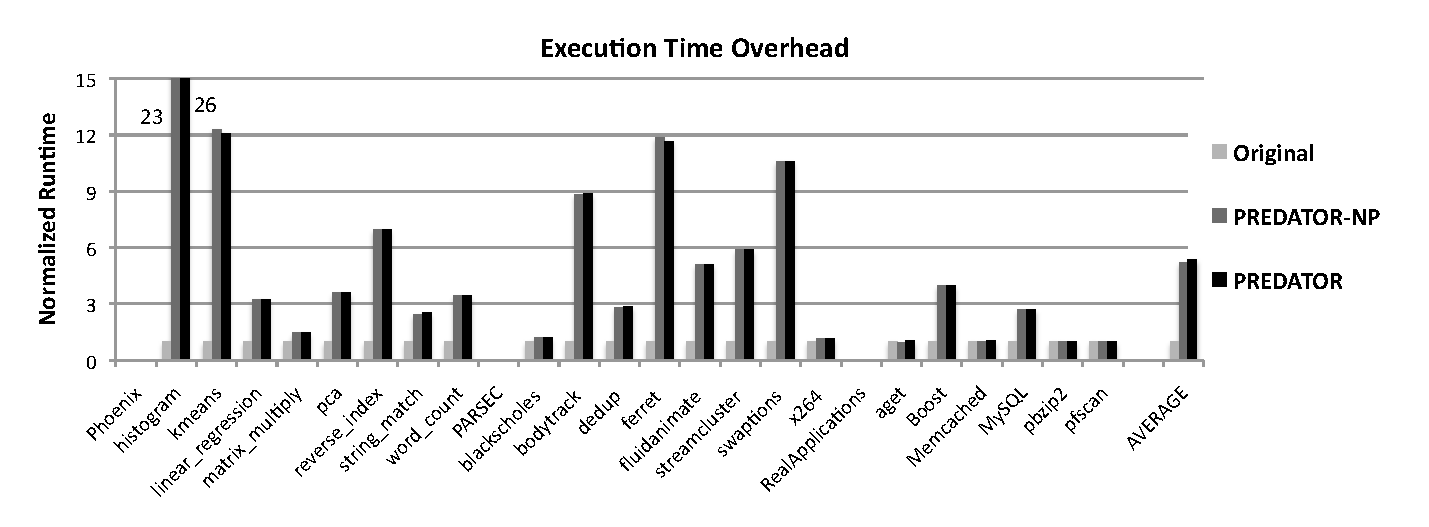
\includegraphics[width=6in]{predator/figure/perf}
\caption{
Performance overhead of \Predator{} with and without prediction(PREDATOR-NP).
\label{fig:perf}}
\end{figure*}
We perform evaluations on different benchmarks and application $10$ times and show the average of $8$ runs in in Figure~\ref{fig:perf}. To avoid the effect caused by extreme outliers, the maximum and minimum values are excluded here. 

For $16$ benchmarks from the Phoenix and PARSEC benchmark suites and six real applications, \Predator{} imposes $5.4\times$ performance overhead averagely. There is no noticeable difference on performance whether the prediction mechanism is enabled or not. 
 
Among five of these programs, histogram, kmeans, bodytrack, ferret, and swaptions, \predator{} introduces more than $8\times$ performance overhead. The histogram benchmark runs more than $26\times$ slower than the one with \pthreads{}, because tracking detailed access on cache lines with false sharing exacerbates the false sharing effect (see more discussion in Section~\ref{sec:sample}).  For bodytrack and ferret, although there is no false sharing, \Predator{} detects a large amount of cache lines with writes larger than {\it Tracking-Threshold}. Thus, tracking those accessing details for those cache lines imposes significant performance overhead. Currently, we have not identified the exact cause of \Predator{}'s high performance for kmeans.
   
\Predator{} imposes a small performance overhead for IO-bound applications, such as matrix\_multiply, blackscholes, x264, aget, Memcached, pbzip2, and pfscan, since \Predator{} does not add any performance overhead for IO operations.  

\subsection{Memory Overhead}
\label{sec:memoverhead}
We evaluate physical memory overhead of \Predator{}, instead of virtual memory overhead, because \Predator{} allocates 4GB virtual memory for its custom memory allocator beforehand. Proportional set size (PSS) of a specific memory mapping (in \texttt{/proc/self/smaps}) reflects the physical memory increase because of running the current application~\cite{memusage}. Thus, we periodically collect this data and use the sum of different memory mappings as the total physical memory usage of running an application. Figure~\ref{fig:memusage} presents the normalized physical memory usage of running different applications, comparing to that using \pthreads{}. 

\Predator{} imposes less than 50\% memory overhead for 17 out of 22 applications.  For swaptions and aget, \Predator{} introduces more memory overhead because the original memory footprints of them are very small, only $3$ kilobytes. Adding the code of detection, prediction and reporting (constant overhead) contributes to a large ratio of memory overhead. The increase of memory consumption in MySQL, from 132 MB to 512 MB, is due to \Predator{}'s heap organization, which does not aggressively reclaim memory held by individual threads. In all cases where \Predator{}'s imposes substantial memory overhead, the applications continue to comfortably fit into RAM on modern platforms.


\subsection{Sampling Rate Sensitivity}
\label{sec:predatorsensitivity}
Section~\ref{sec:sample} describes \Predator{}'s sampling mechanism to reduce tracking overhead. This section evaluates the effect of different sampling rates on performance and effectiveness. Note that running an application with different sampling rates does not affect its memory usage, thus memory overhead is not examined here. 

The default sampling rate used by \Predator{} is 1\%. In this section, we also evaluate two other sampling rates, 0.1\% and 10\%. Figure~\ref{fig:predatorsample} presents performance results under the three different sample rates. We only show the results of those programs having false sharing problems inside, since only their performance are most likely to be affected by different sampling rates. As expected, \Predator{} introduces less performance overhead under a lower sampling rate, but with a very minor performance impact. About effectiveness, even when using the 0.1\% sampling rate, \Predator{} can still detect all false sharing problems, although it reports a lower number of cache invalidations. Thus, different sampling rates do not affect the detection effectiveness.
 
\begin{figure*}[!t]
\centering
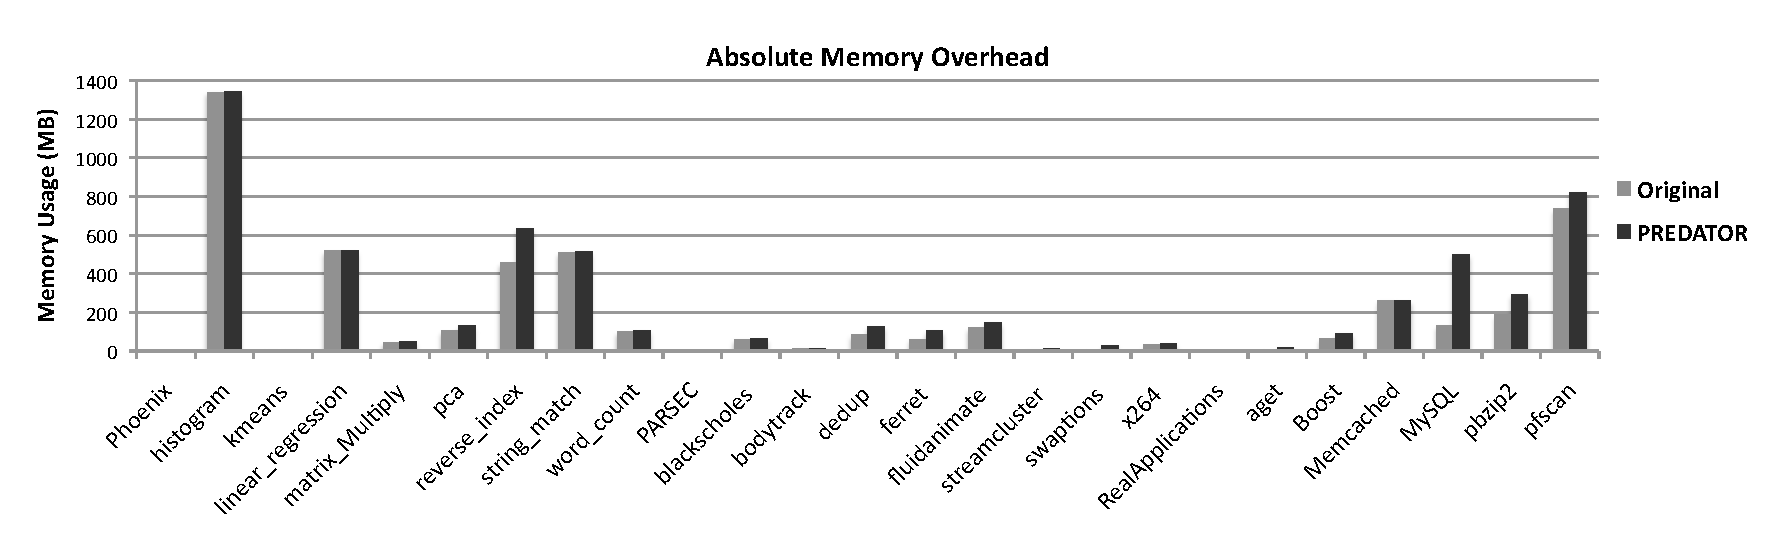
\includegraphics[width=6in]{predator/figure/absolutememory}
\caption{Absolute physical memory usage overhead with \Predator{}.}
\label{fig:absolutememusage}
\end{figure*}

\begin{figure*}[!t]
\centering
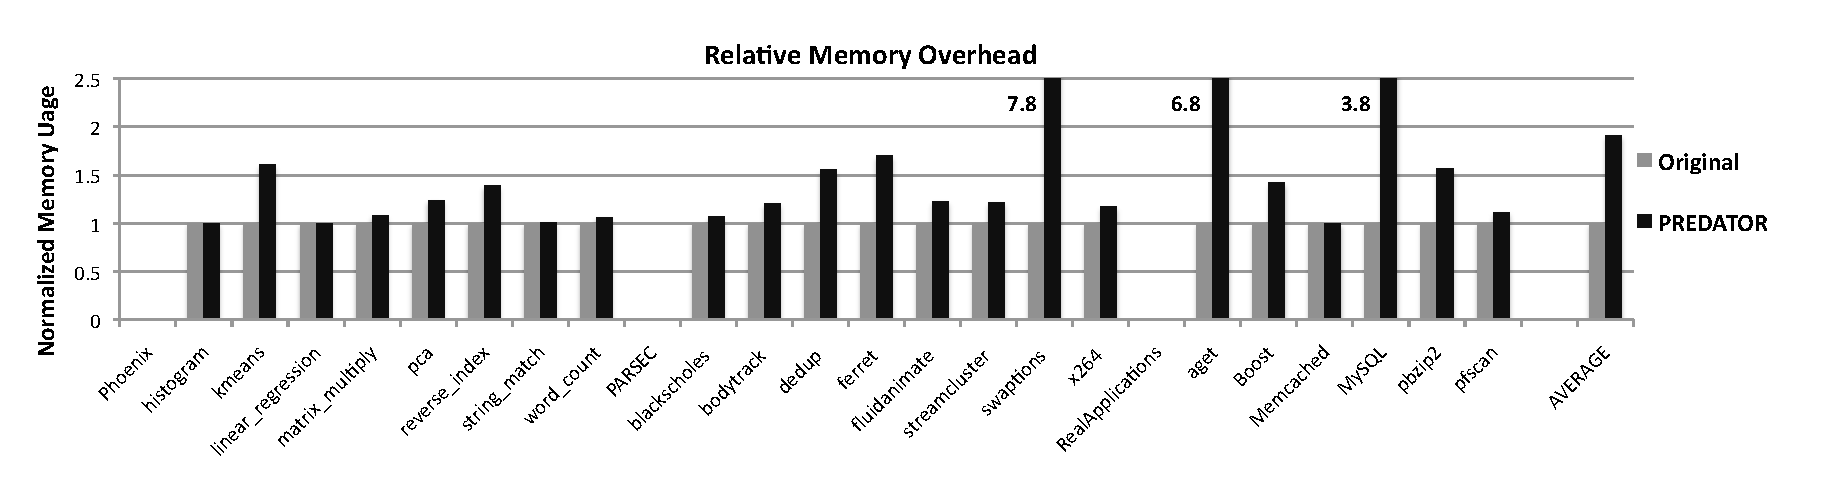
\includegraphics[width=6in]{predator/figure/memusage}
\caption{Relative physical memory usage overhead with \Predator{}.}
\label{fig:memusage}
\end{figure*}

\begin{figure}[!t]
\centering
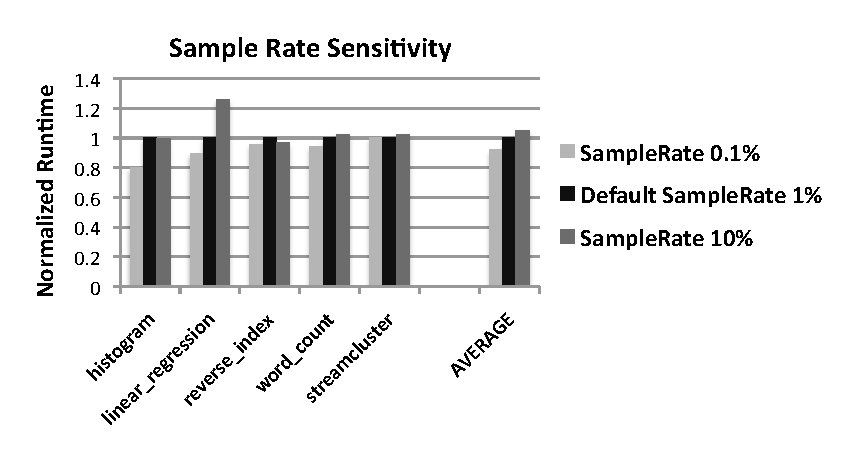
\includegraphics[width=6in]{predator/figure/sample}
%\includegraphics{fig/potential.pdf}
\caption{Sampling rate sensitivity (execution time).}
\label{fig:predatorsample}
\end{figure}




\section{Discussion}
\label{sec:discussion}

\subsection{Instrumentation Selection}
\label{sec:instrumentationtradeoff}
Dynamic binary instrumentation and compiler-based instrumentation are two alternative approaches to perform instrumentation~\cite{Instrumentation}. They exhibit different tradeoffs of performance and generality. Dynamic binary instrumentors, such as Valgrind~\cite{Valgrind}, Pin~\cite{Pin}, and DynamoRIO~\cite{DynamoRIO}, typically analyze the program's code just before execution in order to insert instrumentation. They introduce significant performance overhead, mostly caused by run-time encoding and decoding, but the fact that they operate directly on binaries makes them extremely convenient. By contrast, compiler instrumentation inserts instrumentation in the compilation phase, which requires re-compilation of all source code. 
\Predator{} employs compiler-based instrumentation both because of its better performance and its greater flexibility, as discussed in Section~\ref{sec:selectinstrumentation}.

\subsection{Effectiveness}
Several factors can affect \Predator{}'s ability to identify false sharing.

\emph{Different Inputs.} Different inputs trigger distinct executions of a program. If a specific input does not exercise the code with false sharing problems, \Predator{} cannot necessarily detect them. However, \Predator{} does generalize over inputs to find latent false sharing problems on those exercised code. When any reasonably representative set of inputs are exercised, as is required by any testing regime, \Predator{} can effectively predict false sharing.

\emph{Input Size.} Input size may affect detection results.  As discussed in Section~\ref{optimization}, \Predator{} introduces several threshold values to reduce tracking overhead, which can be adjusted as needed. If the input size is so small that it cannot generate enough false sharing events to cross the pre-defined thresholds, then the detection mechanism will not be triggered. In such cases, \Predator{} will miss actual cases of false sharing. However, realistically large inputs should be enough to trigger \Predator{}'s detection mechanisms. 

\emph{Hardware Independence.}  \Predator{}'s compiler-based approach make it independent of the underlying hardware platform. This approach increases generality, but may lead to over-report false sharing. \Predator{} conservatively assumes that different threads are running on different cores and detects false sharing problems based on possible cache invalidations. However, if multiple threads involved in false sharing are on the same core, then there will be no performance impact. 

%\subsection{Prediction Limitations} 
%\Predator{} can accurately and precisely predict a false sharing problem even when it does not occur. But \Predator{} cannot predict a false sharing problem if the code with false sharing is not exercised at all. Also, \Predator{} may miss potential false sharing problems between two objects brought by a different compiler or memory allocator. 


